\documentclass{standalone}
\usepackage{tikz}
\usepackage{ctex,siunitx}
\setCJKmainfont{Noto Serif CJK SC}
\usepackage{tkz-euclide}
\usepackage{amsmath}
\usetikzlibrary{patterns, calc}
\usetikzlibrary {decorations.pathmorphing, decorations.pathreplacing, decorations.shapes,}
\begin{document}
\small
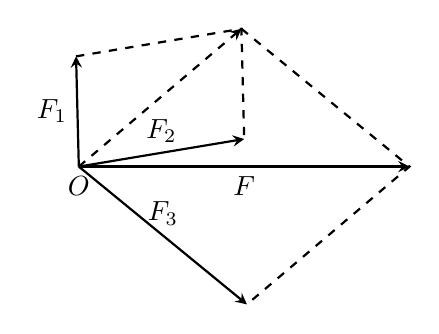
\begin{tikzpicture}[>=stealth, thick,scale=0.7]
  \draw [->] (0,0)node [below]{$O$}--node [below]{$F$}(6,0);
  \draw [->] (0,0)--node [left]{$F_1$}(-.05, 2);
  \draw [->] (0,0)--node [above]{$F_2$}(3, .5);
  \draw [dashed] (-.05, 2)--(-.05+3, 2.5)--(3, .5);
  \draw [dashed] (-.05+3, 2.5)--(6,0)--(6-3+.05, -2.5);
  \draw [->,dashed] (0,0)--(-.05+3, 2.5);
  \draw [->] (0,0)--node [above]{$F_3$} (6-3+.05, -2.5);
\end{tikzpicture}
\end{document}